% Options for packages loaded elsewhere
\PassOptionsToPackage{unicode}{hyperref}
\PassOptionsToPackage{hyphens}{url}
%
\documentclass[
]{article}
\usepackage{amsmath,amssymb}
\usepackage{lmodern}
\usepackage{ifxetex,ifluatex}
\ifnum 0\ifxetex 1\fi\ifluatex 1\fi=0 % if pdftex
  \usepackage[T1]{fontenc}
  \usepackage[utf8]{inputenc}
  \usepackage{textcomp} % provide euro and other symbols
\else % if luatex or xetex
  \usepackage{unicode-math}
  \defaultfontfeatures{Scale=MatchLowercase}
  \defaultfontfeatures[\rmfamily]{Ligatures=TeX,Scale=1}
\fi
% Use upquote if available, for straight quotes in verbatim environments
\IfFileExists{upquote.sty}{\usepackage{upquote}}{}
\IfFileExists{microtype.sty}{% use microtype if available
  \usepackage[]{microtype}
  \UseMicrotypeSet[protrusion]{basicmath} % disable protrusion for tt fonts
}{}
\makeatletter
\@ifundefined{KOMAClassName}{% if non-KOMA class
  \IfFileExists{parskip.sty}{%
    \usepackage{parskip}
  }{% else
    \setlength{\parindent}{0pt}
    \setlength{\parskip}{6pt plus 2pt minus 1pt}}
}{% if KOMA class
  \KOMAoptions{parskip=half}}
\makeatother
\usepackage{xcolor}
\IfFileExists{xurl.sty}{\usepackage{xurl}}{} % add URL line breaks if available
\IfFileExists{bookmark.sty}{\usepackage{bookmark}}{\usepackage{hyperref}}
\hypersetup{
  pdftitle={Appendix: the opportunity of point-of-care diagnostics in general practice: modelling the effects on antimicrobial resistance},
  hidelinks,
  pdfcreator={LaTeX via pandoc}}
\urlstyle{same} % disable monospaced font for URLs
\usepackage[margin=1in]{geometry}
\usepackage{longtable,booktabs,array}
\usepackage{calc} % for calculating minipage widths
% Correct order of tables after \paragraph or \subparagraph
\usepackage{etoolbox}
\makeatletter
\patchcmd\longtable{\par}{\if@noskipsec\mbox{}\fi\par}{}{}
\makeatother
% Allow footnotes in longtable head/foot
\IfFileExists{footnotehyper.sty}{\usepackage{footnotehyper}}{\usepackage{footnote}}
\makesavenoteenv{longtable}
\usepackage{graphicx}
\makeatletter
\def\maxwidth{\ifdim\Gin@nat@width>\linewidth\linewidth\else\Gin@nat@width\fi}
\def\maxheight{\ifdim\Gin@nat@height>\textheight\textheight\else\Gin@nat@height\fi}
\makeatother
% Scale images if necessary, so that they will not overflow the page
% margins by default, and it is still possible to overwrite the defaults
% using explicit options in \includegraphics[width, height, ...]{}
\setkeys{Gin}{width=\maxwidth,height=\maxheight,keepaspectratio}
% Set default figure placement to htbp
\makeatletter
\def\fps@figure{htbp}
\makeatother
\setlength{\emergencystretch}{3em} % prevent overfull lines
\providecommand{\tightlist}{%
  \setlength{\itemsep}{0pt}\setlength{\parskip}{0pt}}
\setcounter{secnumdepth}{5}
\usepackage{booktabs}
\usepackage{longtable}

\ifxetex
  \usepackage{letltxmacro}
  \setlength{\XeTeXLinkMargin}{1pt}
  \LetLtxMacro\SavedIncludeGraphics\includegraphics
  \def\includegraphics#1#{% #1 catches optional stuff (star/opt. arg.)
    \IncludeGraphicsAux{#1}%
  }%
  \newcommand*{\IncludeGraphicsAux}[2]{%
    \XeTeXLinkBox{%
      \SavedIncludeGraphics#1{#2}%
    }%
  }%
\fi
\usepackage{booktabs}
\usepackage{longtable}
\usepackage{array}
\usepackage{multirow}
\usepackage{wrapfig}
\usepackage{float}
\usepackage{colortbl}
\usepackage{pdflscape}
\usepackage{tabu}
\usepackage{threeparttable}
\usepackage{threeparttablex}
\usepackage[normalem]{ulem}
\usepackage{makecell}
\usepackage{xcolor}
\ifluatex
  \usepackage{selnolig}  % disable illegal ligatures
\fi
\usepackage[]{biblatex}
\addbibresource{bibliography-updated.bib}

\title{Appendix: the opportunity of point-of-care diagnostics in general practice: modelling the effects on antimicrobial resistance}
\author{}
\date{\vspace{-2.5em}}

\begin{document}
\maketitle

{
\setcounter{tocdepth}{2}
\tableofcontents
}
\hypertarget{supplemental-methods}{%
\section{Supplemental methods}\label{supplemental-methods}}

MERIAM (Modelling the Economics of Respiratory tract Infections and AMr) is a model built to assess the long-term health-economic effects of improved diagnostics for community-acquired acute respiratory tract infections at the first point of care. The model is developed within the \href{https://value-dx.eu/}{VALUE-Dx} project.

MERIAM has three modules: the demographic module, used to model the population over a long time horizon; the consultation module, used to model patients going to care with an acute respiratory tract infection and the antimicrobial resistance (AMR) forecasting module, used to forecast AMR levels.

The demographic module contains a representative sample of the modeled country. The consultation model uses incidence data to simulate the care-seeking behaviour for community-acquired respiratory tract infections of a subset of individuals from the demographic model and their outcomes, including diagnostics, costs and antibiotic consumption. The AMR module uses antibiotic consumption data to forecast AMR levels.

The time framework of this model is as follows:

\begin{itemize}
\tightlist
\item
  Individuals may seek care for respiratory complaints, with associated costs and health outcomes (in this case mainly prescriptions of antibiotics). The incidence depends on the time of the year (e.g.~there will be an annual peak in the Winter).
\item
  Annually, assess the impact of AMR, based on the consumption of antibiotics.
\item
  Annually, demographic changes (mortality, births, migration) is applied.
\item
  Repeat for 10 years.
\end{itemize}

\hypertarget{demographic_model}{%
\subsection{Demographic module}\label{demographic_model}}

Within the model, nodes are created to represent individuals. Populations are based on demographic data from \href{https://ec.europa.eu/eurostat/home}{Eurostat}, mainly incorporating age and sex, and can be made as large as needed. The ID number is an unique identifier of each node; active indicated whether an individual is alive, sex is 0 for male and 1 for female, age is age (0-99).

The population changes over time are made visible using population pyramids, which are included \protect\hyperlink{res_demographics}{here}. See an example with 10 individuals below in table \ref{tab:node-example}.

\begin{table}

\caption{\label{tab:node-example}example of ten individuals in the model}
\centering
\begin{tabular}[t]{r|r|r|r}
\hline
id & active & sex & age\\
\hline
63025177505 & 1 & 0 & 63\\
\hline
78126034538 & 1 & 1 & 78\\
\hline
1014447809 & 1 & 0 & 1\\
\hline
37018239054 & 1 & 0 & 37\\
\hline
52002065591 & 1 & 0 & 52\\
\hline
17035385673 & 1 & 0 & 17\\
\hline
77066923022 & 1 & 0 & 77\\
\hline
5022297465 & 1 & 0 & 5\\
\hline
22078060602 & 1 & 0 & 22\\
\hline
4054148457 & 1 & 0 & 4\\
\hline
\end{tabular}
\end{table}

\hypertarget{annual-demographic-changes}{%
\subsubsection{Annual demographic changes}\label{annual-demographic-changes}}

Every year the population is updated to reflect the Eurostat projections, here we use model cycles of one year. The following is included:

\begin{itemize}
\item
  Mortality
\item
  Ageing
\item
  Fertility
\item
  Migration
\end{itemize}

This effectively means we assume everyone is born and dies on January 1.

\hypertarget{population_mortality}{%
\paragraph{Mortality}\label{population_mortality}}

Mortality is based on the Eurostat mortality probability projections. The mortality probability is sampled for the active nodes of all age groups. A major assumption in the model is that all nodes over 99 are excluded: we do not include centennials in the model. This is mainly due to data availability for this group.

\hypertarget{ageing}{%
\paragraph{Ageing}\label{ageing}}

Ageing is straightforward in that it increases the age with 1 anually.

\hypertarget{fertility}{%
\paragraph{Fertility}\label{fertility}}

Data on births are used from the Eurostat population projections. The number of babies born is related to the population aged 15-45. The births() function takes the node\_list as an input and returns the node\_list with newly-created nodes (babies). See an example here:

\hypertarget{migration}{%
\paragraph{Migration}\label{migration}}

The model accounts for migration by using the Eurostat projections. The Eurostat projections provide total numbers of immigration (positive number) and emigration (negative number) for 2019-2100. In MERIAM this is related to the total population and converted to a rate. This rate is then used to calculate the total number of immigrants and emigrants. This basically assumes that both immigration and emigration increase when the population size increases.

\hypertarget{overview-data-sources}{%
\paragraph{Overview data sources}\label{overview-data-sources}}

For countries within the European Union, the Eurostat \autocite{europeancommissionEurostat} data sources used are displayed in table \ref{tab:data-eurostatpop}. For the United Kingdom, the population projection data from the Office for National Statistics are used.

\begin{table}

\caption{\label{tab:data-eurostatpop}Overview data sources}
\centering
\begin{tabular}[t]{l|l|l}
\hline
Data & Used for & ID\\
\hline
Population projections & Population, sex, age, fertility & proj\_19np\\
\hline
Migration rates & Migration & proj\_19nanmig\\
\hline
Mortality rates & Mortality & proj\_19naasmr\\
\hline
\end{tabular}
\end{table}

\hypertarget{consulation_model}{%
\subsection{Consultation module}\label{consulation_model}}

Each week, a subset of nodes will seek care. These nodes are selected based on real-world incidence data.

\hypertarget{incidence}{%
\subsubsection{Incidence}\label{incidence}}

Incidence is modeled using the Incidence package. Data is from ECDC. Both Acute Respiratory Infection (ARI) and Influenza-Like Illness (ILI) are modeled (if data is available). Incidence data is stratified by the following age groups:

\begin{itemize}
\item
  0-4 years
\item
  5-14 years
\item
  15-64 years
\item
  65 years and over
\end{itemize}

Incidence data is read into R and then converted into an incidence object from the Incidence package. Two exponential models will be created for each year, one where the number of cases increases over time and one where the number cases decrease. This way, an annual peak is created in the influenza season. The function fit\_optim\_split() from the incidence package is used to automatically determine the peak of the influenza season.

At the start of each model run, the exact incidence is calculated using the model for all weeks. See an example in table \ref{tab:example-incidence}for 4 weeks in a model run with 10,000 nodes for the Netherlands.

\begin{table}

\caption{\label{tab:example-incidence}Example of incidence in model (per 10,000 inhabitants), for Influenza-like ilness (ILI) and Acute respiratory-tract infection (ARI), per week}
\centering
\begin{tabular}[t]{l|r|r}
\hline
Week & ILI & ARI\\
\hline
2020-01 & 59 & 319\\
\hline
2020-02 & 60 & 317\\
\hline
2020-03 & 63 & 316\\
\hline
2020-04 & 58 & 328\\
\hline
\end{tabular}
\end{table}

\hypertarget{index-consultation}{%
\subsubsection{Index consultation}\label{index-consultation}}

During the index consultation, a clinician will perform tests, prescribe antibiotics etc. on the individuals seeking care. For all nodes seeking care (as described above), tests and antibiotic prescriptions are sampled.

As far as the tests are not part of the intervention (in the CRP testing scenario, everyone received a CRP test), they are sampled using the PPAS data \autocite{veldenPrimaryCarePatients2021}.

Antibiotics are also sampled using the PPAS data: the proportion of antibiotic prescriptions is stratified by age (two categories: younger than 60 and 60 and older).

\hypertarget{overview-data-sources-1}{%
\subsubsection{Overview data sources}\label{overview-data-sources-1}}

\hypertarget{probabilities}{%
\paragraph{Probabilities}\label{probabilities}}

In table \ref{tab:probabilities-ppas}, the probabilities related to diagnostics and antibiotics are displayed. These data are from the PPAS \autocite{veldenPrimaryCarePatients2021}.

\begin{table}

\caption{\label{tab:probabilities-ppas}Probabilities related to diagnostics and antibiotics for the Netherlands}
\centering
\begin{tabular}[t]{l|l|l}
\hline
Probability & Value & Distribution\\
\hline
Antibiotic prescription (age: 60 and older) & 0.47 [58 - 66] & Beta [alpha - beta]\\
\hline
Antibiotic prescription (age: younger than 60) & 0.28 [54 - 141] & Beta [alpha - beta]\\
\hline
Prescription of amoxicillin & 0.68 [76 - 36] & Beta [alpha - beta]\\
\hline
Prescription of flucloxacillin & 0.05 [6 - 106] & Beta [alpha - beta]\\
\hline
Prescription of amoxiclav & 0.06 [7 - 105] & Beta [alpha - beta]\\
\hline
Prescription of doxycycline & 0.21 [23 - 89] & Beta [alpha - beta]\\
\hline
Prescription of azithromycin & 0.04 [4 - 108] & Beta [alpha - beta]\\
\hline
Prescription of levofloxacin & 0.01 [1 - 111] & Beta [alpha - beta]\\
\hline
Diagnostic: CRP & 0.32 [99 - 213] & Beta [alpha - beta]\\
\hline
\end{tabular}
\end{table}

\hypertarget{costs}{%
\paragraph{Costs}\label{costs}}

For general practitioner (GP) consults, the Dutch costing manual was used \autocite{hakkaart-vanroijenKostenhandleidingMethodologieVan2015}, while for pharmaceuticals, including the delivery costs, Dutch list prices are used \autocite{zorginstituutnederlandMedicijnkosten}. An overview can be found in table \ref{tab:gp-costs}

\begin{table}

\caption{\label{tab:gp-costs}Consult costs used in the model}
\centering
\begin{tabular}[t]{llll}
\toprule
groupname & Item & nl & Reference\\
\midrule
 & GP consult & €35.37 & Costing manual\\
\cmidrule{2-4}
\multirow{-2}{*}{\raggedright\arraybackslash Consults (costs per consult)} & pharmacy fee & €13 & List prices pharmaceuticals\\
\cmidrule{1-4}
 & amoxicillin & €5.56 & List prices pharmaceuticals\\
\cmidrule{2-4}
 & flucloxacillin & €4.76 & List prices pharmaceuticals\\
\cmidrule{2-4}
 & amoxiclav & €7.72 & List prices pharmaceuticals\\
\cmidrule{2-4}
 & doxycycline & €3.15 & List prices pharmaceuticals\\
\cmidrule{2-4}
 & azithromycin & €1.95 & List prices pharmaceuticals\\
\cmidrule{2-4}
\multirow{-6}{*}{\raggedright\arraybackslash Antibiotic types (costs per course)} & levofloxacin & €6.80 & List prices pharmaceuticals\\
\cmidrule{1-4}
Diagnostics & crp & €4.36 & Costing manual\\
\bottomrule
\end{tabular}
\end{table}

\hypertarget{amr-module}{%
\subsection{AMR module}\label{amr-module}}

The AMR model uses a two-step approach. First, the baseline AMR projections are generated, using an ensemble model. This is a data-driven approach where current trends are used to forecast future AMR rates. These baseline projections are then used as for the current-care scenario, where we assume current patterns in AMR will continue in the future. The second step is to incorporate the impact on antibiotic consumption from the diagnostic strategies, in the baseline AMR projections. This uses a more mechanistically-driven approach. The steps are described in more details below.

Within the VALUE-Dx project, we aim to assess the long-term effects of rapid diagnostics on antimicrobial resistance (AMR). The first step in this process is to forecast AMR rates when the status quo is preserved, i.e.~current AMR policies remain, but no additional measures are taken. Predicting antimicrobial resistance (AMR) is a challenging task, as the development and subsequent spread of resistance genes is highly uncertain. Two methods of modelling AMR in the population over time have been identified \autocite{rotheryFrameworkValueAssessment2018}:

\begin{itemize}
\item
  Mechanistic dynamic transmission models, which models the transmission of resistant pathogens through populations, requiring information on the mechanisms of spread of resistant pathogens.
\item
  Statistical forecasting methods, which is a data-driven approach where the underlying mechanisms of resistance is not considered: past trends are used to forecast future AMR rates.
\end{itemize}

Additionally, expert elicitation is a viable method to forecast AMR, which can be combined with these modeling approaches \autocite{colsonQuantifyingUncertaintyFuture2019} .The mechanisms to attain and retain resistance may differ between various pathogens. As we aim to assess the impact of diagnostics for all community-acquired respiratory-tract infections in the population, which can be caused by various pathogens \autocite{ievenAetiologyLowerRespiratory2018} , we considered a mechanistic dynamic transmission model not to be a viable strategy. A statistical forecasting method, comparable to the methods used by Hashiguchi et al.~was used for this study \autocite{hashiguchiResistanceProportionsEight2019} .

Several methods are available for time series forecasting \autocite{hyndmanForecastingPrinciplesPractice2021,galiciaMultistepForecastingBig2019}, but selecting a single `best' model is challenging. Ensemble methods are an often-used technique to improve forecasts: instead of picking one model, several models are used simultaneously and then combined to provide an average. We developed an ensemble model, averaging three models:

\begin{itemize}
\item
  An exponential smoothing (ETS) model, which forecasts future data using weighted averages of past observations. \autocite{hyndmanForecastingPrinciplesPractice2021}
\item
  A random forest, which aggregates many regression trees to estimate the outcome of interest (AMR rates in our case) \autocite{breimanRandomForests2001}. Bagging (bootstrapping and aggregrating) is used, where each decision tree is informed by a random sample, with only a subset of the available regressors, of the original data set. The different trees are grown in parallel, i.e.~new trees are not informed by previous trees.
\item
  An XGBoost model, which also combines many regression trees to estimate the outcome of interest, however, as opposed to random forests, a sequential tree growing algorithm (boosting) is used, where each new tree informs the creation of the next tree \autocite{chenXGBoostScalableTree2016}.
\end{itemize}

\hypertarget{missing-data}{%
\subsubsection{Missing data}\label{missing-data}}

The European consumption and AMR data had some missing data. These were imputed using the Amelia algorithm \autocite{honakerAmeliaIIProgram2011} which allows for time-series-cross-sectional data to be imputed. To incorporate uncertainty in the various forecasts, the imputation algorithm was run 2000 times to incorporate uncertainty.

\hypertarget{forecasts-of-antibiotic-consumption}{%
\subsubsection{Forecasts of antibiotic consumption}\label{forecasts-of-antibiotic-consumption}}

Antibiotic consumption of broad-spectrum penicillins was forecast using an ETS model.

There are different ETS methods. As we considered annual data, we did not consider seasonal components. The trend can be either none, additive, additive damped or multiplicative. Multiplicative trends tend to produce poor forecasts and additive trends can overestimate the trend on the long term \autocite{hyndmanForecastingPrinciplesPractice2021}, hence we considered an additive damped trend. The consumption data were box-cox transformed so that the data resembled a normal distribution. An example is displayed in figure \ref{fig:abx-consum-ets}.

\begin{figure}
\centering
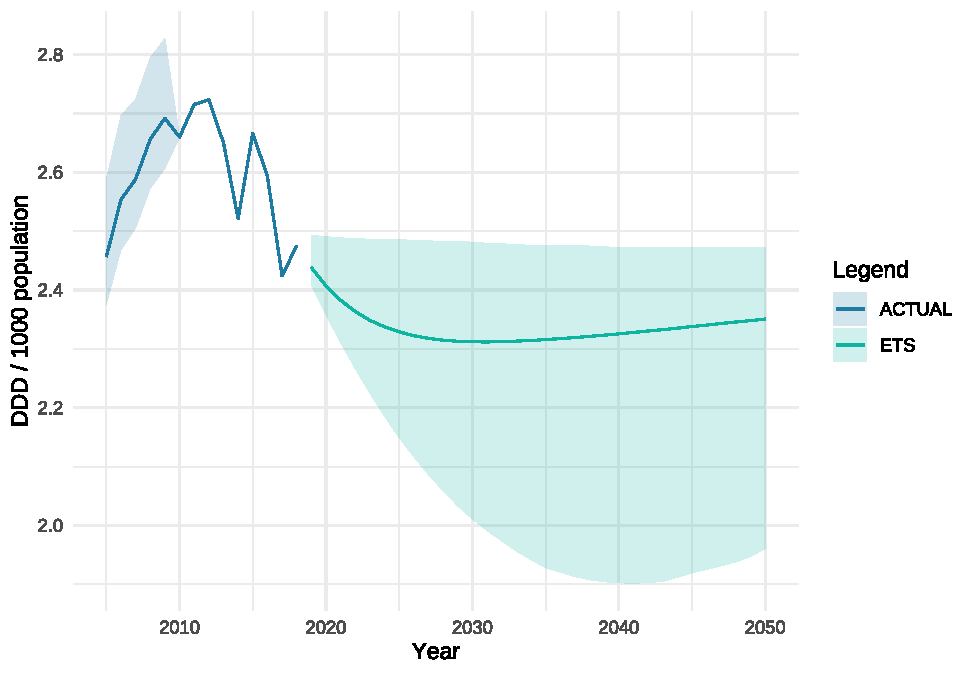
\includegraphics{Appendix_files/figure-latex/abx-consum-ets-1.pdf}
\caption{\label{fig:abx-consum-ets}Antibiotic consumption forecast}
\end{figure}

\hypertarget{amr-forecasts}{%
\subsubsection{AMR forecasts}\label{amr-forecasts}}

For the antimicrobial resistance forecasts the dataset was split into a training and a testing set (training: 2005-2014, testing: 2015-2018), to be able to measure the performance of the forecasts. After fitting the different models to the training set, the prediction of the testing set was assessed. Then the models were refit to the full dataset to forecast the AMR rates up to 2050.

Although we only assessed resistance of \emph{Streptococcus pneumoniae} to broad-spectrum penicillins in the Netherlands in this paper, we incorporated data from other bug-drug combinations and European countries as regressors in the random forest and XGBoost models.

\hypertarget{exponential-smoothing-model}{%
\paragraph{Exponential smoothing model}\label{exponential-smoothing-model}}

The exponential smoothing model uses a similar approach as described for the consumption forecasts, hence an additive, damped, trend.

\hypertarget{random-forest-model}{%
\paragraph{Random forest model}\label{random-forest-model}}

The random forest model uses the following regressors to predict the AMR rate:

\begin{itemize}
\item
  Antibiotic consumption
\item
  GDP forecasts (corrected for purchasing power parities)
\item
  Forecasts proportion population aged \textless{} 15 years
\item
  Forecasts proportion population aged \textgreater{} 64 years
\item
  Forecasts healthcare expenditure (\% of GDP)
\item
  Forecasts out-of-pocket spending on health (\% of total spending on health)
\end{itemize}

The ranger R package was used to build the model \autocite{wrightRangerFastImplementation2017}. The model was tuned to minimize the root mean square error (RMSE), which resulted in a mtry (number of variables included in each bootstrapped sample of 25 and a min.node.size (minimum number of observations in terminal nodes) of 3 \autocite{probstHyperparametersTuningStrategies2019}.

\hypertarget{xgboost-model}{%
\paragraph{XGBoost model}\label{xgboost-model}}

The XGBoost \autocite{chenXGBoostScalableTree2016} model uses the same dependent variables as the random forest model. After tuning the following hyperparameters were chosen:

\begin{itemize}
\item
  min\_child\_weight: 3 (minimum number of instances in child node)
\item
  max\_depth: 11 (maximum depth of each tree)
\item
  eta 0.00920 (learning rate)
\item
  gamma: 0.00158 (mimumum loss reduction to make a further partition on a lead node of the tree)
\end{itemize}

Below are the feature importance plot, an example of a tree used in the XGBoost model and an example of a forecast:

\hypertarget{accuracy-of-predictions}{%
\paragraph{Accuracy of predictions}\label{accuracy-of-predictions}}

The accuracy of the different models is calculated on the testing set, using the models trained only on the training set. Figure \ref{fig:amr-pred-cal} shows an example of the calibration of one model iteration.

\begin{figure}
\centering
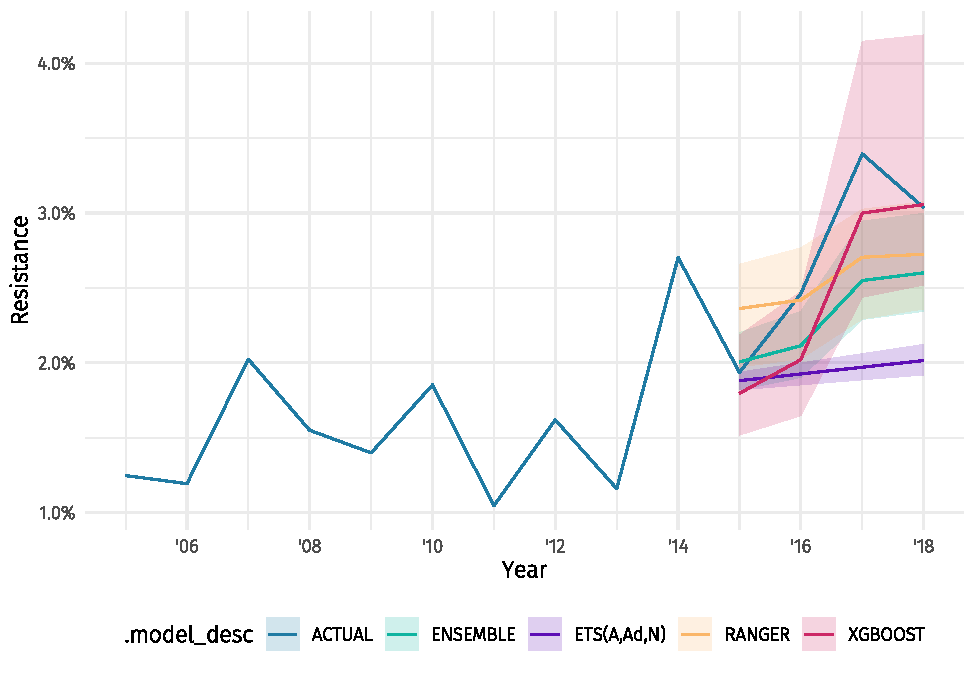
\includegraphics{Appendix_files/figure-latex/amr-pred-cal-1.pdf}
\caption{\label{fig:amr-pred-cal}AMR forecast calibration}
\end{figure}

The performance of time-series forecasts are often represented using the root mean squared error (RMSE), which is calculated using the following formula \autocite{hyndmanForecastingPrinciplesPractice2021}:

\[
RMSE = \sqrt{mean(e^2_t)}
\]

Where \(e_t\) is the forecast error of values from the testing set.

The values differ within the probabilistic analysis, table \ref{tab:amr-accuracy-overview} gives an overview:

\begin{table}[!h]

\caption{\label{tab:amr-accuracy-overview}Overview accuracy metrics AMR predictions}
\centering
\resizebox{\linewidth}{!}{
\begin{tabular}[t]{lllllll}
\toprule
.model\_desc & mae & mape & mase & rmse & rsq & smape\\
\midrule
RANGER & 0.07 [0.04 - 0.11] & 2.8 [1.67 - 4.3] & 0.68 [0.41 - 1.03] & 0.08 [0.05 - 0.12] & 0.6 [0.01 - 0.97] & 2.77 [1.66 - 4.23]\\
XGBOOST & 0.06 [0.03 - 0.11] & 2.34 [1.06 - 4.41] & 0.58 [0.26 - 1.08] & 0.07 [0.03 - 0.12] & 0.88 [0.66 - 0.98] & 2.32 [1.06 - 4.41]\\
ETS & 0.14 [0.12 - 0.17] & 5.57 [4.91 - 6.51] & 1.34 [1.17 - 1.52] & 0.16 [0.15 - 0.19] & 0.76 [0.76 - 0.78] & 5.36 [4.74 - 6.23]\\
\bottomrule
\multicolumn{7}{l}{\rule{0pt}{1em}\textit{Note: }}\\
\multicolumn{7}{l}{\rule{0pt}{1em}mae: mean absolute error; mape: mean absolute percentage error; mase: mean absolute scaled error; root mean square error; rsq: r-squared; smape: symmetric mean absolute percentage error}\\
\end{tabular}}
\end{table}

\hypertarget{forecasts-of-individual-models}{%
\paragraph{Forecasts of individual models}\label{forecasts-of-individual-models}}

Figure \ref{fig:amr-forecasts} gives the AMR forecasts of the individual models.

\begin{figure}
\centering
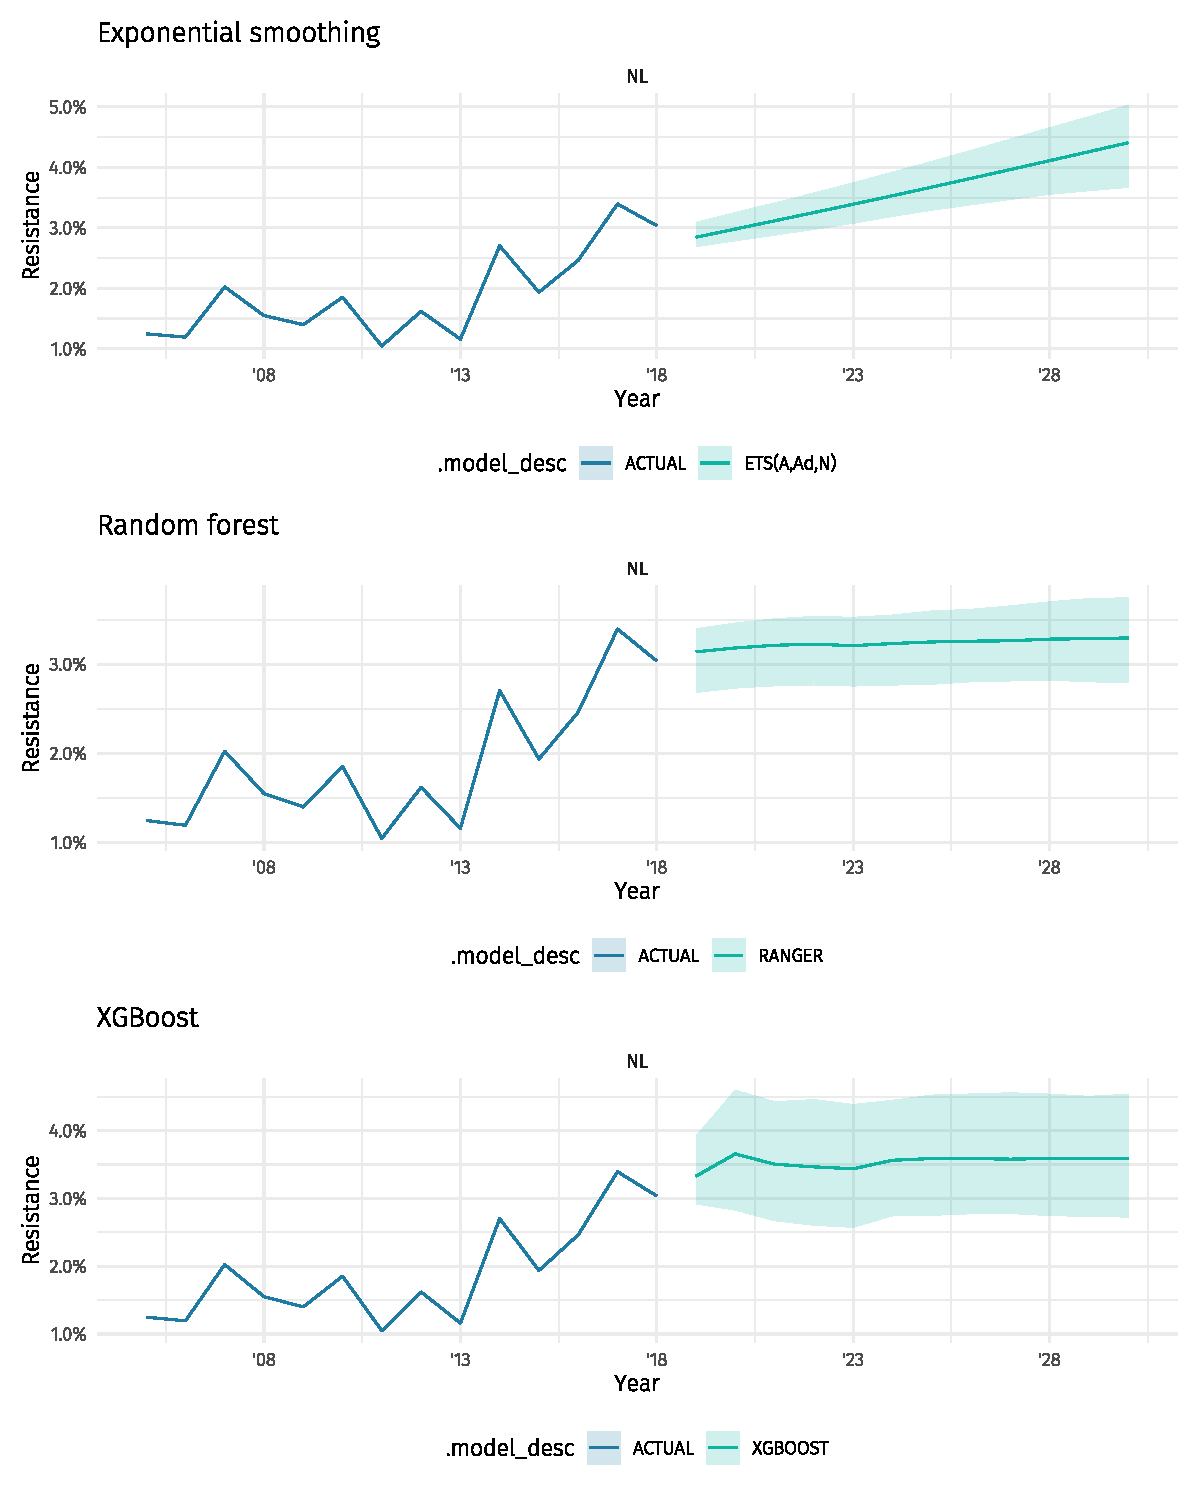
\includegraphics{Appendix_files/figure-latex/amr-forecasts-1.pdf}
\caption{\label{fig:amr-forecasts}Antimicrobial resistance forecasts}
\end{figure}

\hypertarget{ensemble}{%
\paragraph{Ensemble}\label{ensemble}}

The ensemble model is created by averaging (with equal weights) the predicted values across the models. An example is provided in figure \ref{fig:amr-ens}.

\begin{figure}
\centering
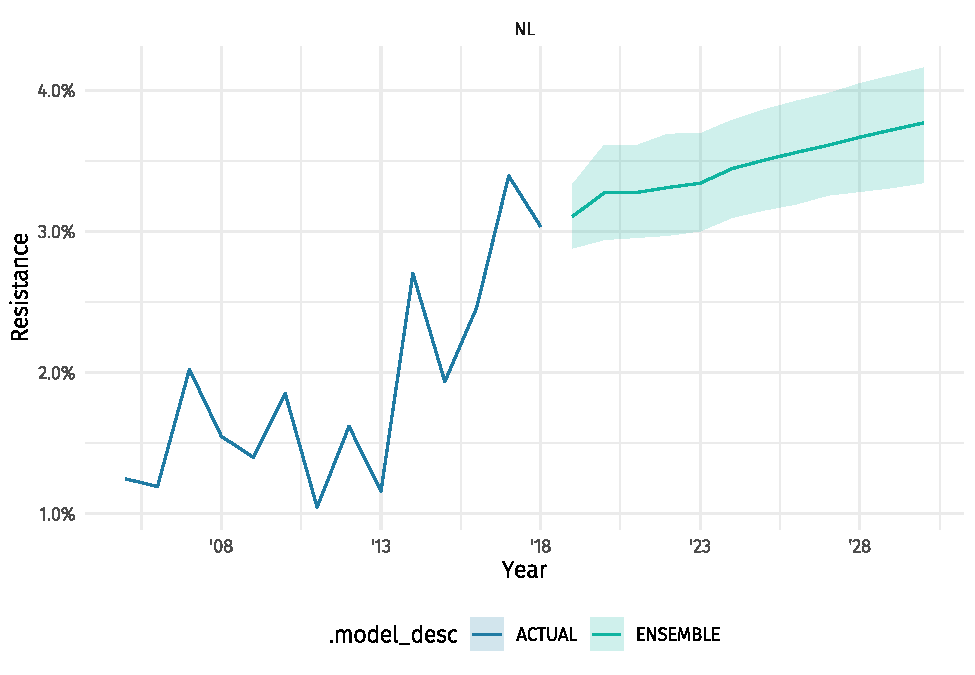
\includegraphics{Appendix_files/figure-latex/amr-ens-1.pdf}
\caption{\label{fig:amr-ens}Ensemble model forecasts}
\end{figure}

\hypertarget{incorporating-uncertainty}{%
\paragraph{Incorporating uncertainty}\label{incorporating-uncertainty}}

The previously described forecasting methods generate point forecasts, that is, a mean is forecast, but no statistical distribution. To incorporate uncertainty in the AMR forecasting model, the following input parameters are varied and the models are fitted for 2000 iterations:

\begin{itemize}
\item
  A different imputed data set is used for both the historical AMR data and antibiotic consumption
\item
  Forecasts healthcare expenditure (\% of GDP) are varied for the model replications
\item
  Forecasts out-of-pocket spending on health (\% of total spending on health) are varied for the model replications
\end{itemize}

Consequently, all model replications use slightly different AMR projections. However, we have not quantified all uncertainty associated with the projections, i.e.~not all possible future AMR rates are included in the modeling.

\hypertarget{incremental-effects-of-diagnostic-strategies}{%
\subsubsection{Incremental effects of diagnostic strategies}\label{incremental-effects-of-diagnostic-strategies}}

As has been described elsewhere, there is a clear relationship between antibiotic consumption and national AMR rates\autocite{goossensOutpatientAntibioticUse2005,cecchiniLowvalueHealthCare2017}. We use this relationship to relate the change in antibiotic consumption, as estimated in MERIAM, to future AMR levels (projected as described above). The following formula is used:

\[
p_{Test,t}^{Ab,B} = p_{Base,t}^{Ab,B} \times \frac{C_{Test,t-1}^{Ab}}{C_{Base,t-1}^{Ab}} \times \epsilon^{Ab,B}
\]

Where \(p_{Test,t}^{Ab,B}\) is the proportion of resistance of bacterium \(B\) to antibiotic \(Ab\) under the testing scenario in the year \(t\); \(p_{Base,t}^{Ab,B}\) the proportion of resistance of bacterium \(B\) to antibiotic \(Ab\) under the base case scenario in the year \(t\); \(C_{Test,t-1}^{Ab}\) the antibiotic consumption of antibiotic \(Ab\) in the year \(t-1\) in the testing scenario; \(C_{Base,t-1}^{Ab}\) the antibiotic consumption of antibiotic \(Ab\) in the year \(t-1\) in the base case scenario and \(\epsilon\) the elasticity between antibiotic consumption of antibiotic \(Ab\) and the development of resistance in bacterium \(B\).

\hypertarget{estimating-elasticity}{%
\paragraph{Estimating elasticity}\label{estimating-elasticity}}

The elasticity \(\epsilon\) is given by the following formula:

\[
\epsilon = \frac{\% \; change \; in \; resistance }{\% \; change \; in \; consumption} 
\]

We calculate the elasticity from the historical antibiotic consumption and resistance data from the ECDC across all countries included in the dataset \autocite{europeancentrefordiseasepreventionandcontrolAntimicrobialResistance2021}. Using ordinary least squares regression on the historical (non-missing) data, a linear function is estimated. See below for the example of the proportion of resistant pneumococci and the consumption of broad-spectrum penicillins:

\begin{figure}
\centering
\includegraphics{figs/elasticity.png}
\caption{Historical consumption of broad spectrum penicillins and resistance of pneumococci}
\end{figure}

This function is then used to estimate the elasticity using the midpoint method, which uses the average percent change of both resistance proportions (\(p\)) and antibiotic consumption (\(C\)) between two points on the linear function:

\[
\epsilon = \frac{\frac{p_2 - p_1}{(p_2 + p_1) / 2} \times 100}{\frac{C_2 - C_1}{(C_2 + C_1) / 2} \times 100} 
\]

The elasticity is not constant, it varies based on the location on the line. To give two examples, a drop from 3 ddd to 2 ddd (daily per 1000 population), a 33\% drop, corresponds to an elasticity of 0.72, resulting in a decline of AMR levels by 24\%. However, a drop from 9 ddd to 6 ddd (also a 33\% drop), corresponds to an elasticity of 0.89, causing an AMR rate decline of 29\%. This also matches prior beliefs, as we would expect a larger influence of antibiotic consumption reductions in countries with a high consumption, compared to countries with a lower consumption. Although antibiotic consumption is the only parameter used here to estimate AMR levels, in reality this is not the only parameter. This is also clear from the graph above, the R\textsuperscript{2} is 0.28, so the correlation is by no means perfect.

\hypertarget{overview-data-sources-2}{%
\subsubsection{Overview data sources}\label{overview-data-sources-2}}

The input data were used based on literature \autocite{hashiguchiResistanceProportionsEight2019} and export opinion, see table \ref{tab:amr-ref} for an overview.

\begin{longtable}[]{@{}
  >{\raggedright\arraybackslash}p{(\columnwidth - 6\tabcolsep) * \real{0.27}}
  >{\raggedright\arraybackslash}p{(\columnwidth - 6\tabcolsep) * \real{0.25}}
  >{\raggedright\arraybackslash}p{(\columnwidth - 6\tabcolsep) * \real{0.17}}
  >{\raggedright\arraybackslash}p{(\columnwidth - 6\tabcolsep) * \real{0.31}}@{}}
\caption{\label{tab:amr-ref} Overview data sources AMR model}\tabularnewline
\toprule
Data & Database & Notes & Reference \\
\midrule
\endfirsthead
\toprule
Data & Database & Notes & Reference \\
\midrule
\endhead
Antimicrobial resistance & Surveillance Atlas for Infectious Disease & & \autocite{europeancentrefordiseasepreventionandcontrolAntimicrobialResistance2021} \\
Antibiotic consumption & ECAC-Net & & \autocite{europeancentrefordiseasepreventionandcontrolAntimicrobialConsumptionDatabase} \\
Population projections & Eurostat & & \autocite{eurostatPopulation1stJanuary2021} \\
Historical demographic data & & & \autocite{eurostatPopulationJanuaryAge2021} \\
GDP projections & OECD & Used for OECD countries & \autocite{oecdLongtermBaselineProjections2018} \\
GDP per capita & World Bank & Used for non-OECD countries & \autocite{theworldbankGDPCapitaPPP} \\
Health expenditure projections & Literature & & \autocite{changPresentFutureGlobal2019} \\
Out-of-pocket healthcare payments projections & Literature & & \autocite{changPresentFutureGlobal2019} \\
\bottomrule
\end{longtable}

\hypertarget{r-environment-and-packages}{%
\subsection{R environment and packages}\label{r-environment-and-packages}}

The current R version in use for MERIAM is R version 4.1.0 (2021-05-18). The Checkpoint package is used to be able to use packages in a reproducible manner, this forces all packages to use the version as published on CRAN on 20 July, 2021.

An overview of the included packages is displayed in table \ref{tab:r-packages}.

\begin{landscape}\begingroup\fontsize{7}{9}\selectfont

\begin{longtable}[t]{lll}
\caption{\label{tab:r-packages}Used packages}\\
\toprule
Package & Version & Authors\\
\midrule
\endfirsthead
\caption[]{\label{tab:r-packages}Used packages \textit{(continued)}}\\
\toprule
Package & Version & Authors\\
\midrule
\endhead

\endfoot
\bottomrule
\endlastfoot
Amelia & 1.8.0 & James Honaker, Gary King, Matthew Blackwell\\
AMR & 1.7.1 & M S Berends, C F Luz, A W Friedrich, B N M Sinha, C J Albers, C Glasner\\
checkpoint & 1.0.0 & Hong Ooi, Andrie de Vries, Microsoft\\
compiler & 4.1.0 & R Core Team\\
countrycode & 1.3.0 & Vincent Arel-Bundock, Nils Enevoldsen, CJ Yetman\\
\addlinespace
dials & 0.0.9 & Max Kuhn\\
doFuture & 0.12.0 & Henrik Bengtsson\\
doRNG & 1.8.2 & Renaud Gaujoux\\
dplyr & 1.0.7 & Hadley Wickham, Romain François, Lionel Henry, Kirill Müller\\
forcats & 0.5.1 & Hadley Wickham\\
\addlinespace
furrr & 0.2.3 & Davis Vaughan, Matt Dancho\\
ggplot2 & 3.3.5 & Hadley Wickham\\
incidence & 1.7.3 & Zhian     , N.        , Kamvar    , Jun       , Cai       , Juliet    , R.C.      , Pulliam   , Jakob     , Schumacher, Thibaut   , Jombart   , Thibaut   , Jombart   , Zhian     , N.        , Kamvar    , Rich      , FitzJohn  , Jun       , Cai       , Sangeeta  , Bhatia    , Jakob     , Schumacher, Juliet    , R.C.      , Pulliam\\
lubridate & 1.7.10 & Garrett Grolemund, Hadley Wickham\\
magrittr & 2.0.1 & Stefan Milton Bache, Hadley Wickham\\
\addlinespace
modeltime & 0.7.0 & Matt Dancho\\
purrr & 0.3.4 & Lionel Henry, Hadley Wickham\\
readr & 1.4.0 & Hadley Wickham, Jim Hester\\
readxl & 1.3.1 & Hadley Wickham, Jennifer Bryan\\
stringr & 1.4.0 & Hadley Wickham\\
\addlinespace
tibble & 3.1.2 & Kirill Müller, Hadley Wickham\\
tidymodels & 0.1.3 & Max Kuhn, Hadley Wickham\\
tidyr & 1.1.3 & Hadley Wickham\\
timetk & 2.6.1 & Matt Dancho, Davis Vaughan\\
truncnorm & 1.0.8 & Olaf Mersmann, Heike Trautmann, Detlef Steuer, Björn Bornkamp\\
\addlinespace
yaml & 2.2.1 & Jeremy Stephens, Kirill Simonov, Yihui Xie, Zhuoer Dong, Hadley Wickham, Jeffrey Horner, reikoch, Will Beasley, Brendan O'Connor, Gregory R. Warnes\\
gt & 0.3.0 & Richard Iannone, Joe Cheng, Barret Schloerke\\
kableExtra & 1.3.4 & Hao Zhu\\
knitr & 1.33 & Yihui                                  , Xie                                    , aut                                    , cre                                    , <https://orcid.org/0000-0003-0645-5666>, Yihui, Xie  , Yihui, Xie\\
patchwork & 1.1.1 & Thomas Lin Pedersen\\
\addlinespace
reactable & 0.2.3 & Greg Lin\\
rmarkdown & 2.10 & JJ       , Allaire  , Yihui    , Xie      , Jonathan , McPherson, Javier   , Luraschi , Kevin    , Ushey    , Aron     , Atkins   , Hadley   , Wickham  , Joe      , Cheng    , Winston  , Chang    , Richard  , Iannone  , Yihui    , Xie      , J.J.     , Allaire  , Garrett  , Grolemund, Yihui     , Xie       , Christophe, Dervieux  , Emily     , Riederer\\
scales & 1.1.1 & Hadley Wickham, Dana Seidel\\*
\end{longtable}
\endgroup{}
\end{landscape}

\newpage

\hypertarget{supplemental-results}{%
\section{Supplemental results}\label{supplemental-results}}

\hypertarget{supplemental-figures}{%
\subsection{Supplemental figures}\label{supplemental-figures}}

Figure \ref{fig:res-demographics} details the demographic development of the population. The example is from one model replication for illustration purposes, there may be small differences between the various model runs. Figure \ref{fig:res-incidence} displays the incidence of respiratory tract infections in the modelled years.

\begin{figure}
\centering
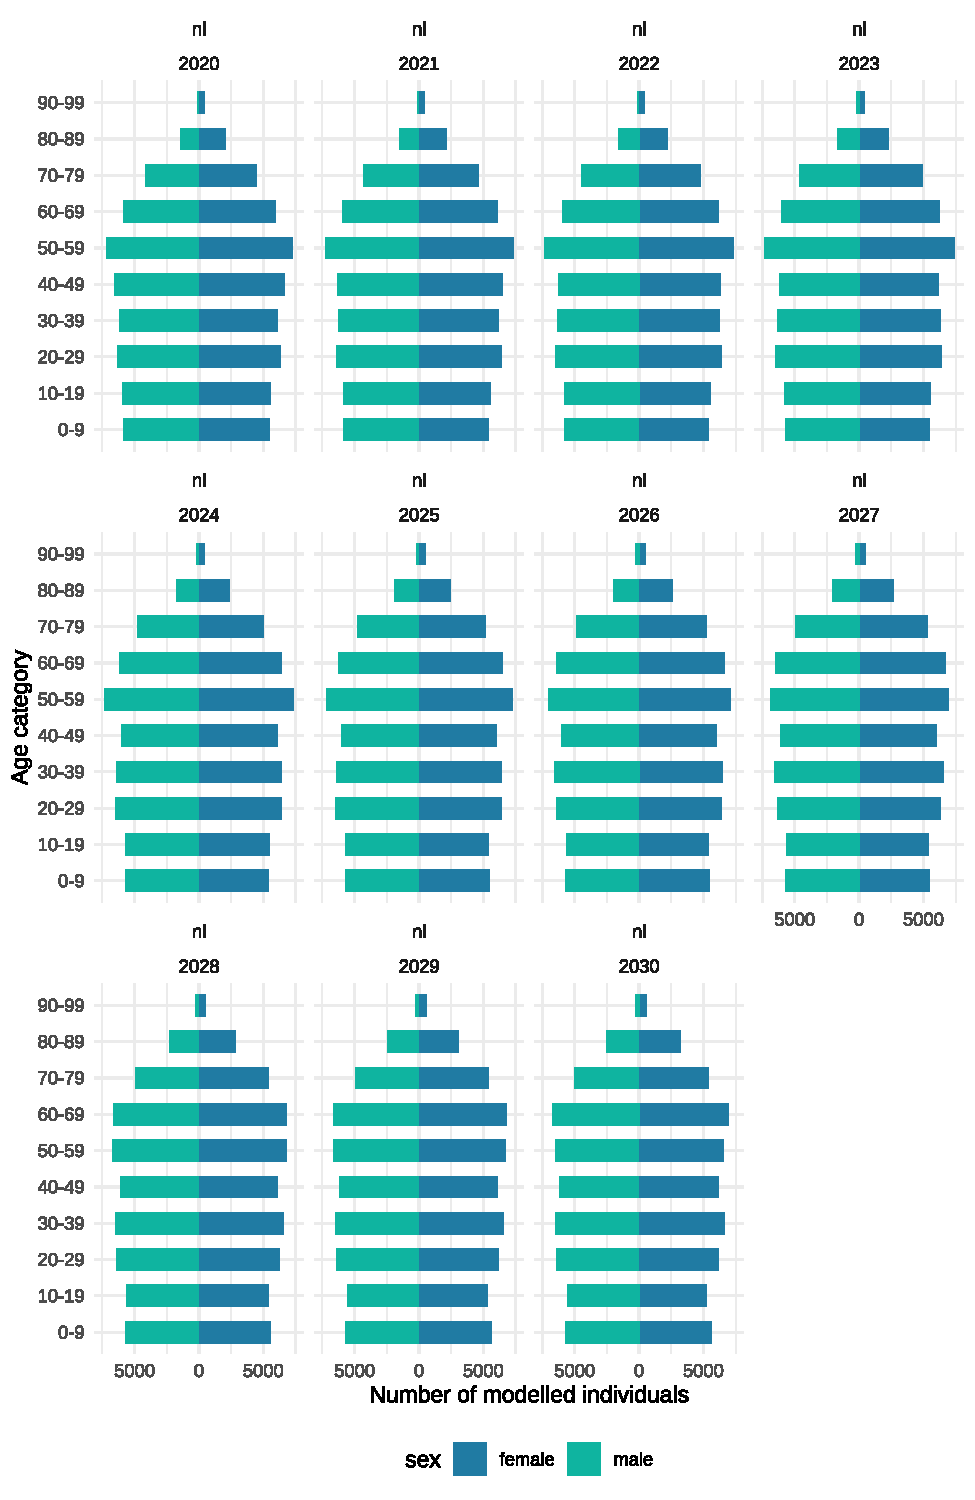
\includegraphics{Appendix_files/figure-latex/res-demographics-1.pdf}
\caption{\label{fig:res-demographics}Demographic projections}
\end{figure}

\begin{figure}
\centering
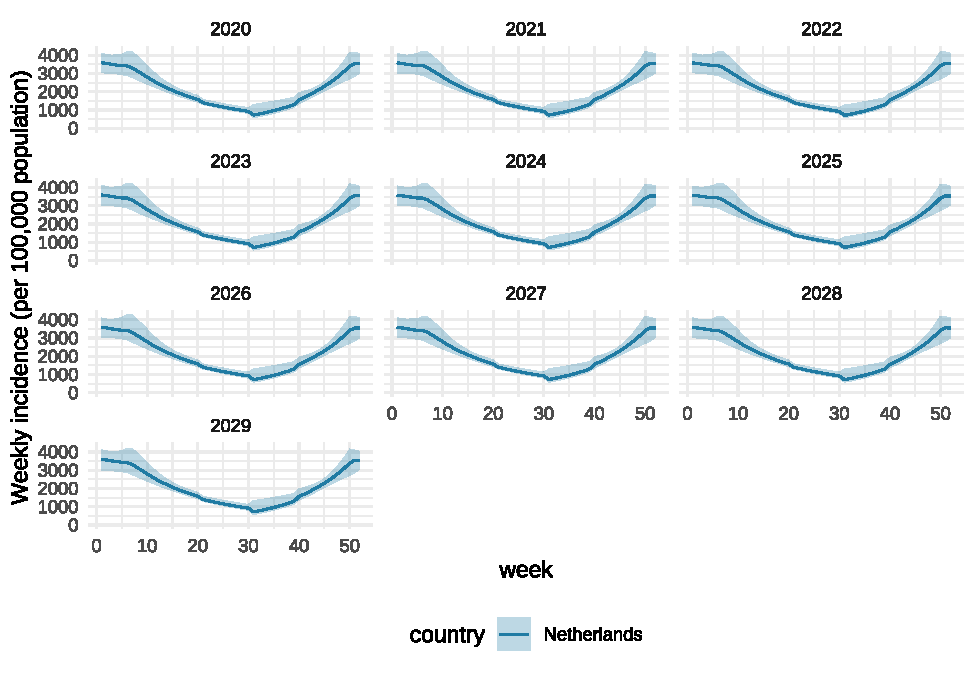
\includegraphics{Appendix_files/figure-latex/res-incidence-1.pdf}
\caption{\label{fig:res-incidence}Incidence projections}
\end{figure}

\hypertarget{supplemental-tables}{%
\subsection{Supplemental tables}\label{supplemental-tables}}

Table \ref{tab:undiscounted-costs} displays the same costs as Table 1 of the main paper, however, the costs are not discounted. In table \ref{tab:total-costs} are all costs (not discounted), grouped by year, shown are the median and the 95\% credible intervals. Displayed in table \ref{tab:ab-consum} is the median annual antibiotic consumption in defined daily dosages, including the 95\% credible intervals, for the different classes of antibiotics.

\begin{verbatim}
## `summarise()` has grouped output by 'country', 'name'. You can override using the `.groups` argument.
\end{verbatim}

\begin{verbatim}
## `summarise()` has grouped output by 'country'. You can override using the `.groups` argument.
\end{verbatim}

\begingroup\fontsize{7}{9}\selectfont

\begin{longtable}[t]{llll}
\caption{\label{tab:undiscounted-costs}Undiscounted costs}\\
\toprule
Cost type & Current standard-of-care & Incremental costs conservative scenario & Incremental costs uncertain scenario\\
\midrule
antibiotics & €1,031,870 (€853,496 - €1,231,761) & -€196,510 (-€393,191 - €9,879) & -€197,375 (-€389,453 - €14,205)\\
consults & €6,079,643 (€5,464,075 - €6,800,547) & €0 (-€248 - €248) & €0 (-€248 - €248)\\
diagnostics & €236,757 (€195,815 - €285,837) & €1,550,974 (€1,387,462 - €1,739,797) & €775,928 (€684,646 - €881,291)\\
total & €7,345,854 (€6,599,496 - €8,212,296) & €1,354,946 (€1,108,864 - €1,625,343) & €576,952 (€374,786 - €818,117)\\
\bottomrule
\end{longtable}
\endgroup{}

\begin{landscape}\begingroup\fontsize{7}{9}\selectfont

\begin{longtable}[t]{llrlll}
\caption{\label{tab:total-costs}Total costs}\\
\toprule
 & Cost category & Year & Current standard-of-care & Incremental costs conservative scenario & Incremental costs uncertain scenario\\
\midrule
\endfirsthead
\caption[]{\label{tab:total-costs}Total costs \textit{(continued)}}\\
\toprule
Country & Cost category & Year & Current standard-of-care & Incremental costs conservative scenario & Incremental costs uncertain scenario\\
\midrule
\endhead

\endfoot
\bottomrule
\endlastfoot
\addlinespace[0.3em]
\multicolumn{6}{l}{\textbf{Netherlands}}\\
\hspace{1em} & antibiotics & 2020 & €98,927 [€80,748 - €121,655) & -€6,970 [-€14,309 - €452) & -€7,037 [-€14,180 - €577)\\
\cmidrule{3-6}\nopagebreak
\hspace{1em} &  & 2021 & €100,085 [€81,806 - €121,925) & -€14,078 [-€28,685 - €801) & -€14,197 [-€28,568 - €1,328)\\
\cmidrule{3-6}\nopagebreak
\hspace{1em} &  & 2022 & €100,946 [€82,426 - €122,625) & -€21,309 [-€42,891 - €1,267) & -€21,584 [-€42,683 - €1,776)\\
\cmidrule{3-6}\nopagebreak
\hspace{1em} &  & 2023 & €101,740 [€83,423 - €124,198) & -€21,391 [-€43,341 - €1,225) & -€21,652 [-€43,498 - €1,771)\\
\cmidrule{3-6}\nopagebreak
\hspace{1em} &  & 2024 & €102,598 [€83,511 - €124,812) & -€21,604 [-€43,501 - €965) & -€21,826 [-€43,291 - €1,735)\\
\cmidrule{3-6}\nopagebreak
\hspace{1em} &  & 2025 & €103,779 [€85,151 - €126,518) & -€21,806 [-€44,372 - €1,068) & -€22,020 [-€43,983 - €1,686)\\
\cmidrule{3-6}\nopagebreak
\hspace{1em} &  & 2026 & €104,483 [€85,915 - €128,356) & -€22,128 [-€44,151 - €1,136) & -€22,167 [-€43,549 - €1,477)\\
\cmidrule{3-6}\nopagebreak
\hspace{1em} &  & 2027 & €105,302 [€86,371 - €127,343) & -€22,279 [-€44,574 - €1,313) & -€22,407 [-€44,522 - €1,394)\\
\cmidrule{3-6}\nopagebreak
\hspace{1em} &  & 2028 & €106,292 [€87,245 - €128,584) & -€22,343 [-€44,654 - €1,021) & -€22,594 [-€44,502 - €1,565)\\
\cmidrule{3-6}\nopagebreak
\hspace{1em} &  & 2029 & €107,190 [€88,346 - €130,770) & -€22,577 [-€45,641 - €1,207) & -€22,763 [-€45,222 - €1,695)\\
\cmidrule{2-6}\nopagebreak
\hspace{1em} & consults & 2020 & €589,836 [€523,098 - €677,554) & €0 [€0 - €0) & €0 [€0 - €0)\\
\cmidrule{3-6}\nopagebreak
\hspace{1em} &  & 2021 & €594,327 [€526,071 - €682,186) & €0 [€0 - €0) & €0 [€0 - €0)\\
\cmidrule{3-6}\nopagebreak
\hspace{1em} &  & 2022 & €597,545 [€532,024 - €680,660) & €0 [-€70.73 - €70.73) & €0 [-€70.73 - €70.73)\\
\cmidrule{3-6}\nopagebreak
\hspace{1em} &  & 2023 & €600,445 [€533,424 - €688,881) & €0 [-€70.73 - €70.73) & €0 [-€70.73 - €70.73)\\
\cmidrule{3-6}\nopagebreak
\hspace{1em} &  & 2024 & €604,636 [€536,219 - €687,741) & €0 [-€70.73 - €70.73) & €0 [-€70.73 - €70.73)\\
\cmidrule{3-6}\nopagebreak
\hspace{1em} &  & 2025 & €608,031 [€539,366 - €694,777) & €0 [-€70.73 - €70.73) & €0 [-€70.73 - €70.73)\\
\cmidrule{3-6}\nopagebreak
\hspace{1em} &  & 2026 & €610,242 [€546,297 - €711,726) & €0 [-€70.73 - €70.73) & €0 [-€70.73 - €70.73)\\
\cmidrule{3-6}\nopagebreak
\hspace{1em} &  & 2027 & €615,211 [€548,700 - €705,861) & €0 [-€35.37 - €35.37) & €0 [-€35.37 - €35.37)\\
\cmidrule{3-6}\nopagebreak
\hspace{1em} &  & 2028 & €617,987 [€548,700 - €705,491) & €0 [-€35.37 - €35.37) & €0 [-€35.37 - €35.37)\\
\cmidrule{3-6}\nopagebreak
\hspace{1em} &  & 2029 & €622,107 [€553,037 - €711,327) & €0 [-€35.37 - €35.37) & €0 [-€35.37 - €35.37)\\
\cmidrule{2-6}\nopagebreak
\hspace{1em} & diagnostics & 2020 & €23,017 [€18,821 - €28,431) & €55,762 [€49,064 - €64,111) & €27,861 [€24,205 - €32,437)\\
\cmidrule{3-6}\nopagebreak
\hspace{1em} &  & 2021 & €23,129 [€18,947 - €28,710) & €112,351 [€99,170 - €129,228) & €56,196 [€48,689 - €65,231)\\
\cmidrule{3-6}\nopagebreak
\hspace{1em} &  & 2022 & €23,336 [€19,126 - €28,427) & €168,888 [€149,326 - €194,352) & €84,487 [€73,912 - €97,618)\\
\cmidrule{3-6}\nopagebreak
\hspace{1em} &  & 2023 & €23,412 [€18,987 - €28,758) & €169,828 [€150,441 - €195,466) & €84,839 [€74,115 - €98,778)\\
\cmidrule{3-6}\nopagebreak
\hspace{1em} &  & 2024 & €23,578 [€19,244 - €29,050) & €171,038 [€151,430 - €195,176) & €85,529 [€74,784 - €98,473)\\
\cmidrule{3-6}\nopagebreak
\hspace{1em} &  & 2025 & €23,776 [€19,423 - €29,235) & €172,132 [€152,445 - €198,415) & €86,038 [€75,054 - €99,662)\\
\cmidrule{3-6}\nopagebreak
\hspace{1em} &  & 2026 & €23,807 [€19,645 - €29,303) & €172,619 [€154,322 - €201,320) & €86,298 [€75,544 - €101,611)\\
\cmidrule{3-6}\nopagebreak
\hspace{1em} &  & 2027 & €23,997 [€19,606 - €29,461) & €173,965 [€153,753 - €200,665) & €86,912 [€75,855 - €100,968)\\
\cmidrule{3-6}\nopagebreak
\hspace{1em} &  & 2028 & €24,145 [€19,693 - €29,617) & €174,836 [€154,598 - €200,623) & €87,614 [€76,582 - €101,425)\\
\cmidrule{3-6}\nopagebreak
\hspace{1em} &  & 2029 & €24,245 [€19,846 - €29,853) & €175,895 [€155,536 - €202,182) & €88,005 [€76,484 - €102,273)\\
\cmidrule{2-6}\nopagebreak
\hspace{1em} & total & 2020 & €711,678 [€631,498 - €819,865) & €48,833 [€39,813 - €59,371) & €20,774 [€13,272 - €29,781)\\
\cmidrule{3-6}\nopagebreak
\hspace{1em} &  & 2021 & €717,041 [€634,380 - €823,261) & €98,161 [€80,443 - €119,990) & €41,904 [€27,104 - €60,114)\\
\cmidrule{3-6}\nopagebreak
\hspace{1em} &  & 2022 & €721,508 [€640,555 - €821,419) & €147,685 [€120,819 - €179,305) & €62,911 [€40,637 - €89,973)\\
\cmidrule{3-6}\nopagebreak
\hspace{1em} &  & 2023 & €725,564 [€642,850 - €834,457) & €148,541 [€121,078 - €181,563) & €63,193 [€40,494 - €91,189)\\
\cmidrule{3-6}\nopagebreak
\hspace{1em} &  & 2024 & €730,940 [€645,972 - €835,152) & €149,624 [€120,408 - €181,958) & €63,656 [€41,563 - €89,975)\\
\cmidrule{3-6}\nopagebreak
\hspace{1em} &  & 2025 & €735,248 [€653,697 - €844,661) & €150,481 [€121,781 - €184,809) & €64,130 [€40,880 - €90,766)\\
\cmidrule{3-6}\nopagebreak
\hspace{1em} &  & 2026 & €738,955 [€658,911 - €857,975) & €151,379 [€122,515 - €185,395) & €64,276 [€41,212 - €93,208)\\
\cmidrule{3-6}\nopagebreak
\hspace{1em} &  & 2027 & €745,136 [€662,878 - €853,358) & €152,371 [€123,449 - €185,219) & €64,802 [€41,729 - €92,113)\\
\cmidrule{3-6}\nopagebreak
\hspace{1em} &  & 2028 & €748,365 [€663,752 - €854,892) & €152,693 [€123,909 - €186,273) & €65,158 [€41,730 - €93,102)\\
\cmidrule{3-6}\nopagebreak
\hspace{1em} &  & 2029 & €753,571 [€667,230 - €860,840) & €153,625 [€124,108 - €185,946) & €65,272 [€41,760 - €93,877)\\*
\end{longtable}
\endgroup{}
\end{landscape}

\begin{landscape}\begingroup\fontsize{7}{9}\selectfont

\begin{longtable}[t]{llrlll}
\caption{\label{tab:ab-consum}Annual antibiotic consumption}\\
\toprule
 & Antibiotic class & Year & Current standard-of-care & Conservative scenario & Uncertain scenario\\
\midrule
\endfirsthead
\caption[]{\label{tab:ab-consum}Annual antibiotic consumption \textit{(continued)}}\\
\toprule
Country & Antibiotic class & Year & Current standard-of-care & Conservative scenario & Uncertain scenario\\
\midrule
\endhead

\endfoot
\bottomrule
\endlastfoot
\addlinespace[0.3em]
\multicolumn{6}{l}{\textbf{Netherlands}}\\
\hspace{1em} & Amoxicillin/clavulanic acid & 2020 & 3297 (1396 - 6174) & 3108 (1670 - 5187) & 3118 (1669 - 5260)\\
\cmidrule{3-6}\nopagebreak
\hspace{1em} &  & 2021 & 3350 (1449 - 6332) & 2898 (1606 - 4725) & 2888 (1596 - 4882)\\
\cmidrule{3-6}\nopagebreak
\hspace{1em} &  & 2022 & 3350 (1375 - 6353) & 2662 (1091 - 5072) & 2646 (1186 - 5145)\\
\cmidrule{3-6}\nopagebreak
\hspace{1em} &  & 2023 & 3370 (1438 - 6374) & 2656 (1102 - 5114) & 2656 (1176 - 5271)\\
\cmidrule{3-6}\nopagebreak
\hspace{1em} &  & 2024 & 3412 (1428 - 6594) & 2698 (1112 - 5124) & 2678 (1155 - 5334)\\
\cmidrule{3-6}\nopagebreak
\hspace{1em} &  & 2025 & 3454 (1480 - 6636) & 2740 (1134 - 5229) & 2709 (1176 - 5344)\\
\cmidrule{3-6}\nopagebreak
\hspace{1em} &  & 2026 & 3486 (1448 - 6678) & 2730 (1124 - 5250) & 2751 (1208 - 5419)\\
\cmidrule{3-6}\nopagebreak
\hspace{1em} &  & 2027 & 3518 (1501 - 6720) & 2762 (1102 - 5367) & 2782 (1218 - 5366)\\
\cmidrule{3-6}\nopagebreak
\hspace{1em} &  & 2028 & 3560 (1460 - 6552) & 2788 (1124 - 5272) & 2793 (1228 - 5502)\\
\cmidrule{3-6}\nopagebreak
\hspace{1em} &  & 2029 & 3580 (1522 - 6815) & 2835 (1144 - 5292) & 2824 (1239 - 5492)\\
\cmidrule{2-6}\nopagebreak
\hspace{1em} & Broad-spectrum penicillins & 2020 & 37406 (29894 - 46778) & 34786 (28728 - 42433) & 34766 (28811 - 42842)\\
\cmidrule{3-6}\nopagebreak
\hspace{1em} &  & 2021 & 37674 (30208 - 47484) & 32424 (26438 - 39932) & 32487 (26533 - 40173)\\
\cmidrule{3-6}\nopagebreak
\hspace{1em} &  & 2022 & 38084 (30260 - 47859) & 30104 (22994 - 38946) & 30046 (23476 - 39407)\\
\cmidrule{3-6}\nopagebreak
\hspace{1em} &  & 2023 & 38398 (30491 - 48196) & 30408 (23089 - 39470) & 30324 (23551 - 39376)\\
\cmidrule{3-6}\nopagebreak
\hspace{1em} &  & 2024 & 38756 (30990 - 48575) & 30660 (23329 - 39419) & 30644 (23708 - 39820)\\
\cmidrule{3-6}\nopagebreak
\hspace{1em} &  & 2025 & 39070 (31195 - 48837) & 30912 (23488 - 39902) & 30812 (23886 - 40113)\\
\cmidrule{3-6}\nopagebreak
\hspace{1em} &  & 2026 & 39501 (31499 - 49162) & 31174 (23654 - 40059) & 31180 (24212 - 40826)\\
\cmidrule{3-6}\nopagebreak
\hspace{1em} &  & 2027 & 39806 (31626 - 49529) & 31490 (23772 - 40868) & 31426 (24475 - 40951)\\
\cmidrule{3-6}\nopagebreak
\hspace{1em} &  & 2028 & 39989 (32056 - 49729) & 31794 (24233 - 40961) & 31647 (24664 - 41118)\\
\cmidrule{3-6}\nopagebreak
\hspace{1em} &  & 2029 & 40462 (32389 - 50959) & 32036 (24191 - 41509) & 31804 (24863 - 41638)\\
\cmidrule{2-6}\nopagebreak
\hspace{1em} & Narrow-spectrum penicillins & 2020 & 3752 (1512 - 7561) & 3528 (1890 - 6314) & 3570 (1778 - 6315)\\
\cmidrule{3-6}\nopagebreak
\hspace{1em} &  & 2021 & 3822 (1526 - 7672) & 3346 (1736 - 5699) & 3304 (1722 - 5810)\\
\cmidrule{3-6}\nopagebreak
\hspace{1em} &  & 2022 & 3822 (1498 - 7756) & 3038 (1176 - 6328) & 2996 (1162 - 5978)\\
\cmidrule{3-6}\nopagebreak
\hspace{1em} &  & 2023 & 3843 (1540 - 7770) & 3066 (1204 - 6328) & 3052 (1134 - 6105)\\
\cmidrule{3-6}\nopagebreak
\hspace{1em} &  & 2024 & 3871 (1568 - 7896) & 3122 (1204 - 6300) & 3080 (1134 - 6146)\\
\cmidrule{3-6}\nopagebreak
\hspace{1em} &  & 2025 & 3906 (1582 - 7883) & 3136 (1218 - 6357) & 3122 (1162 - 6216)\\
\cmidrule{3-6}\nopagebreak
\hspace{1em} &  & 2026 & 3983 (1638 - 7981) & 3185 (1232 - 6552) & 3122 (1106 - 6412)\\
\cmidrule{3-6}\nopagebreak
\hspace{1em} &  & 2027 & 3976 (1582 - 7994) & 3206 (1190 - 6482) & 3150 (1176 - 6300)\\
\cmidrule{3-6}\nopagebreak
\hspace{1em} &  & 2028 & 4011 (1624 - 8316) & 3192 (1246 - 6608) & 3164 (1162 - 6384)\\
\cmidrule{3-6}\nopagebreak
\hspace{1em} &  & 2029 & 4046 (1652 - 8303) & 3206 (1260 - 6735) & 3178 (1204 - 6440)\\
\cmidrule{2-6}\nopagebreak
\hspace{1em} & Macrolides/lincosamides & 2020 & 619 (176 - 1447) & 598 (252 - 1184) & 590 (248 - 1188)\\
\cmidrule{3-6}\nopagebreak
\hspace{1em} &  & 2021 & 630 (173 - 1462) & 558 (241 - 1062) & 551 (238 - 1069)\\
\cmidrule{3-6}\nopagebreak
\hspace{1em} &  & 2022 & 630 (184 - 1476) & 497 (155 - 1174) & 493 (148 - 1196)\\
\cmidrule{3-6}\nopagebreak
\hspace{1em} &  & 2023 & 637 (176 - 1483) & 504 (158 - 1217) & 490 (140 - 1192)\\
\cmidrule{3-6}\nopagebreak
\hspace{1em} &  & 2024 & 644 (191 - 1505) & 508 (166 - 1217) & 500 (144 - 1217)\\
\cmidrule{3-6}\nopagebreak
\hspace{1em} &  & 2025 & 644 (191 - 1501) & 518 (158 - 1206) & 504 (151 - 1224)\\
\cmidrule{3-6}\nopagebreak
\hspace{1em} &  & 2026 & 652 (191 - 1530) & 518 (162 - 1199) & 504 (144 - 1224)\\
\cmidrule{3-6}\nopagebreak
\hspace{1em} &  & 2027 & 666 (198 - 1509) & 520 (169 - 1217) & 515 (155 - 1246)\\
\cmidrule{3-6}\nopagebreak
\hspace{1em} &  & 2028 & 664 (191 - 1530) & 529 (162 - 1224) & 513 (148 - 1264)\\
\cmidrule{3-6}\nopagebreak
\hspace{1em} &  & 2029 & 666 (194 - 1555) & 531 (166 - 1242) & 522 (151 - 1253)\\
\cmidrule{2-6}\nopagebreak
\hspace{1em} & Quinolones & 2020 & 158 (10 - 864) & 168 (19 - 629) & 170 (19 - 662)\\
\cmidrule{3-6}\nopagebreak
\hspace{1em} &  & 2021 & 163 (10 - 878) & 158 (19 - 534) & 168 (19 - 566)\\
\cmidrule{3-6}\nopagebreak
\hspace{1em} &  & 2022 & 168 (10 - 874) & 120 (5 - 669) & 130 (10 - 672)\\
\cmidrule{3-6}\nopagebreak
\hspace{1em} &  & 2023 & 163 (10 - 882) & 120 (5 - 662) & 130 (10 - 682)\\
\cmidrule{3-6}\nopagebreak
\hspace{1em} &  & 2024 & 163 (10 - 907) & 120 (5 - 654) & 134 (5 - 678)\\
\cmidrule{3-6}\nopagebreak
\hspace{1em} &  & 2025 & 173 (10 - 883) & 125 (5 - 679) & 134 (5 - 696)\\
\cmidrule{3-6}\nopagebreak
\hspace{1em} &  & 2026 & 168 (10 - 921) & 120 (5 - 677) & 134 (10 - 720)\\
\cmidrule{3-6}\nopagebreak
\hspace{1em} &  & 2027 & 175 (10 - 932) & 130 (5 - 696) & 134 (5 - 696)\\
\cmidrule{3-6}\nopagebreak
\hspace{1em} &  & 2028 & 173 (10 - 923) & 125 (8 - 699) & 134 (8 - 702)\\
\cmidrule{3-6}\nopagebreak
\hspace{1em} &  & 2029 & 178 (10 - 922) & 125 (5 - 691) & 134 (10 - 716)\\
\cmidrule{2-6}\nopagebreak
\hspace{1em} & Tetracyclines & 2020 & 7441 (5019 - 10640) & 6951 (5061 - 9373) & 6937 (5047 - 9451)\\
\cmidrule{3-6}\nopagebreak
\hspace{1em} &  & 2021 & 7525 (5026 - 10710) & 6528 (4816 - 8701) & 6503 (4711 - 8883)\\
\cmidrule{3-6}\nopagebreak
\hspace{1em} &  & 2022 & 7602 (5110 - 10710) & 6006 (3913 - 8716) & 5978 (4039 - 8918)\\
\cmidrule{3-6}\nopagebreak
\hspace{1em} &  & 2023 & 7648 (5187 - 10822) & 6076 (4011 - 8828) & 6072 (3997 - 8940)\\
\cmidrule{3-6}\nopagebreak
\hspace{1em} &  & 2024 & 7690 (5292 - 10934) & 6132 (4011 - 8800) & 6125 (3997 - 9011)\\
\cmidrule{3-6}\nopagebreak
\hspace{1em} &  & 2025 & 7784 (5271 - 11054) & 6195 (4081 - 9031) & 6153 (4074 - 9198)\\
\cmidrule{3-6}\nopagebreak
\hspace{1em} &  & 2026 & 7882 (5367 - 11180) & 6272 (4130 - 9108) & 6216 (4108 - 9353)\\
\cmidrule{3-6}\nopagebreak
\hspace{1em} &  & 2027 & 7931 (5389 - 11200) & 6314 (4151 - 9199) & 6265 (4158 - 9310)\\
\cmidrule{3-6}\nopagebreak
\hspace{1em} &  & 2028 & 7994 (5390 - 11340) & 6370 (4102 - 9185) & 6307 (4130 - 9352)\\
\cmidrule{3-6}\nopagebreak
\hspace{1em} &  & 2029 & 8046 (5425 - 11431) & 6440 (4220 - 9289) & 6363 (4186 - 9471)\\*
\end{longtable}
\endgroup{}
\end{landscape}

\newpage

\printbibliography[title=References]

\end{document}
